\section{Covering Spaces}

In this section, we outline the basics of covering space theory and explore ways in which covering spaces can help us compute and understand fundamental groups.

Let's begin by appealing to some intuition from our proof that the fundamental group of the circle. A key idea was lifting a loop in the circle into a path from the real line to the circle. We observed that the condition of being homotopically trivial corresponded precisely to the condition of the endpoints of the path in $\R$ lying in the same $\Z$-translate of the fundamental domain. This intuition can be developed and formalised into a much more comprehensive theory.

\subsection{Definition and First Examples}

Throughout this chapter, let $X$ be a topological space.

\begin{boxdefinition}[Covering (Space/Map)]
    A space $\Tilde{X}$ along with a map $p : \Tilde{X} \to X$ is called a \textbf{covering space of $X$} if the following are all true:
    \begin{enumerate}
        \item $p$ is surjective
        \item There is an open covering $\U$ of $X$ such that for all $U \in \U$, there exist open sets $V_{\alpha} \ssq \Tilde{X}$ such that
        \begin{enumerate}
            \item The $V_{\alpha}$ are all disjoint
            \item $p\inv[U] = \bigcup_{\alpha} V_{\alpha}$
            \item $p\rest{V_{\alpha}} : V_{\alpha} \to U$ is a homeomorphism
        \end{enumerate}
    \end{enumerate}
    We refer to $\Tilde{X}$ as a \textbf{covering space} and $p$ as a \textbf{covering map}.
\end{boxdefinition}

First, a concrete example.

\begin{boxexample}[$\R$ covers $S^1$]
    $\R$, along with the map $p : \R \to S^1 : t \mapsto e^{2\pi i t}$, is a covering space of $S^1$.
\end{boxexample}

Next, a handwavy example.

\begin{boxexample}[The Torus covers the Torus]
    You can `unravel' the torus into `two tori stuck together' to form a covering space of the torus.
    \begin{figure}[H]
        \centering
        \begin{subfigure}{0.45\linewidth}
            \centering
            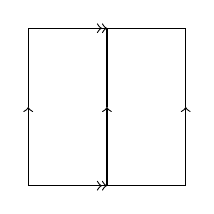
\begin{tikzpicture}
                \draw[->] (-1, -1) -- (-1, 0);
                \draw[-] (-1, 0) -- (-1, 1);
                \draw[->] (0, -1) -- (0, 0);
                \draw[-] (0, 0) -- (0, 1);
                \draw[->] (1, -1) -- (1, 0);
                \draw[-] (1, 0) -- (1, 1);
                \draw[->>] (-1, 1) -- (0, 1);
                \draw[-] (0, 1) -- (1, 1);
                \draw[->>] (-1, -1) -- (0, -1);
                \draw[-] (0, -1) -- (1, -1);
            \end{tikzpicture}
        \end{subfigure}
        \hfill
        \begin{subfigure}{0.45\linewidth}
            \centering
            \begin{tikzpicture}
                \draw[->] (-1, -1) -- (-1, 0);
                \draw[-] (-1, 0) -- (-1, 1);
                \draw[->] (1, -1) -- (1, 0);
                \draw[-] (1, 0) -- (1, 1);
                \draw[->>] (-1, 1) -- (0, 1);
                \draw[-] (0, 1) -- (1, 1);
                \draw[->>] (-1, -1) -- (0, -1);
                \draw[-] (0, -1) -- (1, -1);
            \end{tikzpicture}
        \end{subfigure}
        \caption{A depiction of what's going on}
    \end{figure}
\end{boxexample}

We will see that if a space has a nontrivial fundamental group, then it is the quotient of some space by its fundamental group. Moreover, we will see that this action is ``properly discontinuous'' and that the parent space, along with the quotient map, form a covering space. So the notion of fundamental groups is fundamentally linked to the notion of covering spaces.

As a side note, we define simply connected spaces.

\begin{boxdefinition}[Simply Connected Space]
    We say that a path-connected space $X$ is \textbf{simply connected} if $\pi_1(X)=0$.
\end{boxdefinition}

What our above remark tells us about simply connected spaces is that they admit no covering spaces that are acted on properly discontinuously by a (nontrivial) group.

\subsection{Lifting Theorems}

In this subsection, we give two types of (path-)lifting theorems. The first lifts paths (between points) and the second lifts homotopies (paths between paths).

\begin{boxtheorem}[Path Lifting Theorem]
    Let $p : \Tilde{X} \to X$ be a covering of $X$. Pick a basepoint $\Tilde{x_0} \in \Tilde{X}_0$ and $x_0 \in X$ so that $p\of{\Tilde{x_0}} = x_0$ (i.e. having fixed a basepoint $x_0\in X$, we choose any $\tilde{x_0}\in p^{-1}(x_0)$ as a basepoint of $\tilde{X}$). Let $\gamma : I \to X$ be a path, with $\gamma(0) = x_0$. There is a unique path $\Tilde{\gamma} : I \to \Tilde{X}$ such that $p \circ \Tilde{\gamma} = \gamma$ and $\Tilde{\gamma}\of{0} = \tilde{x_0}$.
    \begin{cd*}
        & \Tilde{X} \arrow[d, "p"] \\[1em]
        I \arrow[ur, "\Tilde{\gamma}"] \arrow[r, "\gamma"'] & X
    \end{cd*}
\end{boxtheorem}
\begin{proof}[Proof (see also \sorry)]
    Let $\U$ be a family of evenly covered sets in $X$. Let $\V = \setst{\gamma\inv[U]}{U \in \U}$. This is an open cover of $I$. Since $I$ is compact, this admits a finite subcover. Thus\footnote{If I have \textit{any} finite open cover of the unit interval, I can find finitely many such $t_i$, and I can choose them so that each interval $\brac{t_i, t_{i + 1}}$ is contained in an element of that open cover - just draw a picture.}, there are $0 = t_0 < t_1 < \cdots < t_n = 1$ with $\gamma\of{\brac{t_i, t_{i + 1}}} \ssq U$ for some $U \in \U$.

    Inductively, if $\Tilde{\gamma}$ has been defined on $\brac{0, t_i}$, we can extend $\Tilde{\gamma}$ by $\parenth{p\rest{\Tilde{U}}}\inv \circ \gamma\rest{\brac{t_i, t_{i + 1}}}$, where $\Tilde{U}$ is the connected component of $p\inv[U]$ containing $\Tilde{\gamma}\of{t_i}$.

    Uniqueness is ``by intuition'' (i.e. the path is uniquely defined on each set of $\V$, and then since $\V$ covers $I$ uniqueness of $\tilde{\gamma}$ should follow with no additional trouble).
\end{proof}

We can now do the same for paths between paths.

\begin{boxtheorem}[Homotopy Lifting Theorem]
    Let $p : \Tilde{X} \to X$ be a covering of $X$. Pick a basepoint $\Tilde{x_0} \in \Tilde{x}$ and $x_0 \in X$ so that $p\of{\Tilde{x_0}} = x_0$. Let $F : I \times I \to X$ be a homotopy of paths starting at $x_0 \in X$. There is a unique homotopy $\Tilde{F} : I \times I \to \Tilde{X}$ lifting $F$ (that is, $p \circ \Tilde{F} = F$) with $\Tilde{F}\of{0, 0} = \Tilde{x_0}$.
\end{boxtheorem}
The paths between which $F$ is a homotopy are precisely
\begin{align*}
    \gamma : I \to X : t \mapsto F(t, 0)
    \delta : I \to X : t \mapsto F(t, 1)
\end{align*}
and the paths between which $\Tilde{F}$ is a homotopy are the unique lifts $\Tilde{\gamma}, \Tilde{\delta} : I \to \Tilde{X}$ given by the path-lifting theorem.
\begin{proof}[Proof sketch]
    Let $\U$ be an open cover of $X$. Split $I \times I$ into finitely many rectangles $R_{ij}$ such that $F\!\brac{R_{ij}} \ssq U$ for some $U \in \U$. Construct $\Tilde{F}$ by inverting $p$ on the corresponding $U$ and composing with $\Tilde{F}$.
\end{proof}

Given all of this, we can now prove that indeed $\pi_1(S^1)=\Z$ in a simpler/cleaner (if equivalent) way.

\begin{boxtheorem}
    $\pi_1(S^1)=\Z$
\end{boxtheorem}
\begin{proof}
    Having already shown (earlier in these notes) that for $\gamma$ such that $[\gamma]\in \pi_1(S^1)$, letting $\gamma_n:I\rightarrow S^1$ such that $\gamma_n:x\mapsto e^{2\pi i nx}$ (for some $n\in \Z$) then we must have $[\gamma]=[\gamma_n]$ for some $n$, we let $H:I\times I \rightarrow S^1$ be a homotopy from $\gamma_n$ to $\gamma_0$. We can now lift $H$ to some $\tilde{H}:I\times I \rightarrow \R$, and we'll have $\tilde{H}(\cdot, 0)$ will be a lift of $\gamma_n$ to $\tilde{H}(1,0)=0$, $\tilde{H}(1,1)=n$...\sorry
\end{proof}

\subsection{Fundamental Groups of Covering Spaces}

There is an immediate (and very strong) statement we can make about the fundamental group of a covering space.

\begin{boxtheorem}
    If $p : \Tilde{X} \to X$ is a covering with $p\of{\Tilde{x_0}} = x_0$, then the induced map $p_{\#} : \pi_1\of{\Tilde{X}, \Tilde{x_0}} \to \pi_1\of{X, x_0}$ is injective.
\end{boxtheorem}
\begin{proof}
    \sorry (should follow because path-lifting is unique)
    % Something about deformation retractions?
\end{proof}

An immediate consequence is that if a space has trivial fundamental group, so must any covering space of it. That is,

\begin{boxcorollary}
    If $X$ is simply-connected, then every covering space of $X$ is also simply-connected.
\end{boxcorollary}

But in fact, we can say something even stronger.

\begin{boxdefinition}[One-Sheetedness of a Covering]
    We say that a covering $p:\Tilde{X}\rightarrow X$ is one-sheeted if $p^{-1}(x)$ has cardinality 1 for all $x\in X$.% Idea - only one sheet for any point and nbhd
\end{boxdefinition}

\begin{boxproposition}
    Let $X$ be a simply-connected space (and, in particular, path-connected) space and let $p : \Tilde{X} \to X$ be a covering. Then, $p$ is one-sheeted.
\end{boxproposition}
\begin{proof}
    Suppose not. Fix some $x_0 \in X$ and suppose that $p\inv\of{x_0}$ has two distinct points $\Tilde{x_1}$ and $\Tilde{x_2}$. Let $\tg : I \to \TX$ be a path from $\txi$ to $\txii$. Let $\gamma = p \circ \tg$. This is a loop at $x_0$. Let $\gamma_t$ be a homotopy from $\gamma_0 = \gamma$ and $\gamma_1 = c_{x_0}$, the constant path at $x_0$. We know there is a unique lifted homotopy $\tg_t$. This is a homotopy from $c_{\txi}$ (and also from $c_{\txii}$) to $\tg$ with fixed endpoints, so $\tg$ has to be a loop, meaning $\txi = \txii$.
\end{proof}

In particular, a simply-connected space $X$ can have no non-trivial path-connected covering space. 

Our next goal will be to show that path-connected covering spaces of $X$, up to an appropriate notion of equivalence, are in bijection with subgroups of the fundamental group. See also \cite[Ch 5, \S 8 « Correspondance galoisienne »]{EPFLTopologie}.

% [TODO] say something about how the number of sheets above one point is the same as the number of sheets above another point (presumably because of path-connectedness?)

\begin{boxtheorem}
    Let $p : \TX \to X$ be a covering, with $p\of{\txo} = x_0$. Suppose $\TX$ and $X$ are path-connected. Then the number of sheets of $p$ is equal to the index of $p_{\#}\!\brac{\pi_1\of{\TX, \txo}}$ in $\pi_1\of{X, x_0}$.
\end{boxtheorem}
\begin{proof}
    For the purposes of this proof, denote
    \begin{align*}
        G = \pi_1\of{X, x_0}
        \qquad \qquad
        H = p_{\#}\!\brac{\pi_1\of{\TX, \txo}}
    \end{align*}
    We can define a map from the set of right-cosets of $H$ to the fibre of $x_0$ by
    \begin{align*}
        \phi : \setst{Hg}{g \in G} \to p\inv\of{x_0} : H\brac{\gamma} \mapsto \tg\of{1}
    \end{align*}
    We need to show that $\phi$ is well-defined.
    \begin{itemize}
        \item \underline{Well-definedness in terms of homotopy class:} If $\gamma$ and $\delta$ are such that $\brac{\gamma} = \brac{\delta} \in G$, then we have a unique lifted homotopy from (the lifted paths) $\tilde{\gamma}$ to $\tilde{\delta}$, so they will map to the same element of the fibre (i.e. the lifted paths must end in the same place, as these paths are really loops $\gamma, \delta$ with $[\gamma]= [\delta]\in \pi_1(X,x_0)$). \sorry % some lifting theorem
        
        \item \underline{Well-definedness in terms of cosets:} If $\gamma$ and $\delta$ are non-homotopic paths such that $H\brac{\gamma} = H \brac{\delta}$, then $\tg(1) = \Tilde{\delta}(1)$ because for all $[h] \in H$, $\Tilde{h}$ is a loop in $\TX$ (i.e. $\gamma(1)=\gamma(0)=\delta(1)=\delta(0)=x_0$. Then, because there is a unique lift, if the cosets $H[\gamma]$ and $H[\delta]$ are equal, we must have the translates of the constant path at $x_0$ by $\gamma, \delta$ equal, from which it follows that the lifted paths have the same start/end point). \sorry % more work needed maybe?
    \end{itemize}

    We now claim that $\phi$ is, in fact, a bijection.

    \begin{itemize}
        \item \underline{$\phi$ is surjective:} Fix $\txi \in p\inv\of{x_0}$. Let $\tg$ be a path from $\txo$ to $\txi$. We know $\gamma = p \circ \tg$ is a loop based at $x_0$. In fact,
        \begin{align*}
            \phi\of{H \brac{\gamma}} = \tg(1) = \txi
        \end{align*}

        \item \underline{$\phi$ is injective:} Suppose that $\phi\of{H \brac{\gamma}} = \phi\of{H\brac{\gamma'}}$ - this would imply that $\tilde{\gamma}(1)=\tilde{\gamma'}(1)\implies \gamma, \gamma'$ translate the constant path to the same point ($\tilde{\gamma}(1)=\tilde{\gamma'}(1)$), which implies that the cosets $H[\gamma], H[\gamma']$ must be the same. 
    \end{itemize}
\end{proof}

\begin{boxdefinition}[Semi-Locally Simply-Connected (SLSC)]
    A space $X$ is \textbf{semi-locally simply-connected (SLSC)} if for all $x \in X$, there is some open neighbourhood $U \ni x$ such that the homomorphism $i_{\#} : \pi_1\of{U, x} \to \pi_1\of{X, x}$ induced by the inclusion $i : U \inj X$ is the trivial map.
\end{boxdefinition}

\subsection{Deck Transformations and Universal Covers}

Let $X$ be a topological space and let $p : \TX \to X$ be a covering. We define a notion of `automorphisms of covering spaces'.

\begin{boxdefinition}[Deck Transformation]
    A \textbf{deck transformation} is an automorophsim of $p : \TX \to X$, that is, a homeomorphism $f : \TX \to \TX$ such that $p \circ f = p$, ie, the following diagram commutes:
    \begin{cd*}
        \TX \arrow[rr, "f"] \arrow[dr, "p"'] & & \TX \arrow[dl, "p"] \\
        & X &
    \end{cd*}
    The set of deck transformations forms a group $\Deck{p}$ under composition.
\end{boxdefinition}

We can show the following useful fact.

\begin{boxproposition}
    If $\TX$ is simply connected then $\Deck{p} \cong \pi_1\of{X}$.
\end{boxproposition}

Now that we have a definition of automorphisms of covering spaces, we can define special objects via some universal property.

\begin{boxtheorem}[Existence of Universal Covers]
    Let $X$ be
    \begin{itemize}
        \item path-connected
        \item locally path-connected
        \item SLSC
    \end{itemize}
    Then there is a universal cover $p : \TX \to X$ of $X$.
\end{boxtheorem}
\begin{proof}
    Pick a basepoint $x_0 \in X$. Define $\TX$ to be the following set of homotopy classes (with fixed endpoints):
    \begin{align*}
        \TX = \setst{\brac{\alpha}}{\alpha : I \to X \text{ is a path with } \alpha(0) = x_0}
    \end{align*}
    Define a covering map
    \begin{align*}
        p : \TX \to X : \brac{\alpha} \mapsto \alpha(1)
    \end{align*}
    This is well-defined (ie, doesn't depend on the homotopy class) because the homotopy classes are taken with fixed endpoints.

    \sorry
\end{proof}

\begin{boxlemma}
    Let $p:\tilde{X}\rightarrow X$ be a covering space with $p(\tilde{x_0})=x_0$ and let $f:Y\rightarrow X$ with $f(y_0)=x_0$ with $Y$ a space which is path-connected and locally path-connected. Then a lift $\tilde{f}:Y\rightarrow \tilde{X}$ of $f$ exists is equivalent to the statement that $f_{\#}(\pi_1(Y, y_0))\ssq p_{\#}(\pi_1(\tilde{X}, \tilde{x_0}))$.
\end{boxlemma}
\begin{proof}
    for the forwards direction, $p\circ \tilde{f}=f\implies p_{\#}\circ f_{\#}=f_{\#}\implies \text{im}(f_{\#}\ssq \text{im}(p_{\#})$.

    for the other, we construct $\tilde{f}$. Let $y\in Y$ be arbitrary and let $\gamma$ be a path from $y_0$ to $y$. then $f\circ \gamma$ is a path from $x_0$ to $f(y)$. Lift this path $\tilde{(f\circ \gamma)}:I\rightarrow \tilde{X}$, then we have $\tilde{f}(y)=\tilde{(f\circ \gamma)}(1)$. We want this to be well-defined...
\end{proof}

\begin{boxlemma}
    If $X$ is path-connected and locally path-connected with $p_1:\tilde{X_1}\rightarrow X$ and $p_2:\tilde{X_2}\rightarrow X$ a path-connected covering space of $X$, then $p_1, p_2$ are isomorphic via $f:\tilde{X_1}\rightarrow \tilde{X_2}$ that maps $\tilde{x_1}\in p_1^{-1}(x_0)$ to $\tilde{x_2}\in p_2^{-1}(x_0)$ (or equivalently we will have that $(p_1)_{\#}(\pi_1(\tilde{X_1}, x_1))=(p_2)_{\#}(\pi_1(\tilde{X_2}, \tilde{x_2}))$.)
\end{boxlemma}
\begin{proof}
    for the forwards direction $p_2\circ f=p_1\implies (p_2)_{\#}\circ f_{\#}=(p_1)_{\#}$ and the other way around $\implies \text{im}((p_1)_{\#})=\text{im}((p_2)_{\#})$...\sorry
\end{proof}
To summarize after this last proof (which will one day be completed), $X$ path-connected, locally path-connected and SLSC, then every subgroup $H\leq \pi_1(X, x_0)$ there is \textbf{at most} one covering space $p:\tilde{X}\rightarrow X$ with $p(\tilde{x_0})=x_0$ and $H=p_{\#}(\pi_1(\tilde{X}, \tilde{x_0}))$. 

For such $X$ we have constructed a simply connected covering space $p:\tilde{X}\rightarrow X$ and $\pi_1(X, x_0)$ acts on $\tilde{X}$ by deck transformations.
\begin{boxdefinition}[$G$-actions on spaces]
    Let $X$ be a space and $G$ a group, then a ``$G$-action on $X$'' is a homomorphism $G\rightarrow \text{Homeo}(X)$.
\end{boxdefinition}
\begin{boxnotation}
    We say that $g\in G$ induces the homeomorphism $x\mapsto gx$ and $gh:x\mapsto (gh)\cdot x = g(h\cdot x)$
\end{boxnotation}
An example is given if we let $\Z$ act on $\R$ by translation.
\sorry \textcolor{red}{... [teresa - 20ish minutes of class were missed, my apologies]}
\begin{boxdefinition}[Normal Covering Spaces]
    Let $p:\tilde{X}\rightarrow X$ be a covering space. Then we say that $p$ is ``normal'' if $\forall x\in X$ and $\forall \tilde{x_1}, \tilde{x_2}\in p^{-1}(x)$ there is a deck transformation that maps $\tilde{x_1}$ to $\tilde{x_2}$.
\end{boxdefinition}
\begin{boxproposition}
    Normal covering spaces correspond to normal subgroups of $\pi_1(X, x_0)$.
\end{boxproposition}
\begin{proof}
    Let $p: \tilde{X}\rightarrow X$ be a covering space with $\tilde{X}$ path-connected and locally path-connected, let $H=p_{\#}(\pi_1(\tilde{X}, \tilde{x_0}))$. Recall that the ``normalizer'' of $H$ a subgroup of $G$ is given by $N(H):=\{g\in G: gH=Hg\}$ and also recall that $p:\tilde{X}\rightarrow X$ a covering space which is path-connected, then there is a deck transformation $f:\tilde{X}\rightarrow \tilde{X}$ that maps $\tilde{x_0}\in p^{-1}(x_0)$ to $\tilde{x_1}\in p^{-1}(x_0)$. Equivalently, $p_{\#}(\pi_1(\tilde{X}, \tilde{x_0}))=p_{\#}(\pi_1(\tilde{X}, \tilde{x_1}))$. Now $p_{\#}(\pi_1(\tilde{X}, \tilde{x_0}))=H$ and $p_{\#}(\pi_1(\tilde{X}, \tilde{x_1}))=[\gamma]H[\gamma]^{-1}$ where $\gamma=p\circ \alpha$ with $\alpha:I\rightarrow \tilde{X}$ a path from $\tilde{x_0}$ to $\tilde{x_1}$. Thus such a deck transformatition exists iff $[\gamma]\in N(H)$...\sorry
.\end{proof}

\begin{boxtheorem}
    $p:\tilde{X}\rightarrow X$ a covering space with $\tilde{X}$ path connected/locally path-connected, then $\text{Deck}(p)\cong N(H)/H$ where $H=p_{\#}(\pi_1(\tilde{X}, \tilde{x_0}))$.
\end{boxtheorem}
\begin{proof}
    Let $\phi:N(H)\rightarrow\text{Deck}(p)$ with $[\alpha]\mapsto \tau$ where $\tau:\tilde{X}\rightarrow \tilde{X}$ is the deck transformation that maps $\tilde{x_0}=\tilde{\alpha}(0)$ to  $\tilde{x_1}=\tilde{\alpha}(1)$. Note that $\phi$ is a group homomorphism, and $\phi([\gamma][\gamma^{-1}])=\phi([\gamma])\cdot \phi([\gamma^{-1}])=\tau$. Now $\gamma \star \gamma'$ lifts to $\tilde{\gamma}\star \tau \circ \tilde{\gamma'}$ a path from $\tilde{x_0}$ to $\tau(\tilde{x_2})=\tau\circ \tau'(\tilde{x_0})$, the deck transformation that maps $\tilde{x_0}$ to $\tau \circ \tau'(\tilde{x_0})$ is $\tau \circ \tau'$, so $\phi([\alpha])=\id$ iff $\tilde{\gamma}$ is a loop iff $[\alpha]\in H\implies \ker(\phi)=H$...note that the intersection of these two parts is not path-connected.\sorry
\end{proof}

After having developed some theory about covering spaces, we have some algebraic applications:
\begin{boxtheorem}[Nielsen-Schreier Theorem]
    Any subgroup of a free group is free.
\end{boxtheorem}
\begin{proof}
    (sketch) We consider the free group generated by a set $S$ and observe that $F_S$ (the free group on $S$) is isomorphic to $\pi_1(\vee_S S^1$ (a wedge of $S$ circles). Let $H<F_S$, then $H$ corresponds to some covering space $p:X_H\rightarrow X$, let $H=p_{\#}(\pi_1(X_H))$. Since $p$ is a local homeomorphism, $X_H$ is a graph (of vertices and edges). Let $T$ be a maximal tree in $X_H$, then $T$ is contractible and $X_H/T\cong \vee_S S^1$. Now (one can show) $X_H/T\simeq X_H$, so $\pi_1(X_H)$ is free.
\end{proof}
and a classic
\begin{boxtheorem}[Fundamental Theorem of Algebra]
    If $p:\C\rightarrow \C$ is a nonconstant polynomial, $p$ has a 0.
\end{boxtheorem}
\begin{proof}
    Divide everything by its absolute value to get $\hat{p}:\C\rightarrow S^1$, the $\hat{p}$ restricted to $\partial B_r(0)$ (the ball of radius $r$ centered at 0) and to $\partial B_{r-1}(0)$ are homotopic. Now...\sorry
\end{proof}

We also claim that if $G$ is any finitely generated group, then there is a space $X$ with $\pi_1(X)\cong G$. To sketch the proof, we want to let $\tilde{X}=G\star G \star G$ the ``three-fold join of $G$'' which we build as a tri-partite graph with each part having vertices in $G$, and then we glue in a triangle for every choice of point (one from each column). This has a natural $G$-action which is properly discontinuous, and then $X=\tilde{X}/G$...and ``this is the start of group cohomology''...

% My notetaking today has been horrible - apologies. But in a week or two you will probably know why...

